\begin{figure}[htbp]
    \centering
    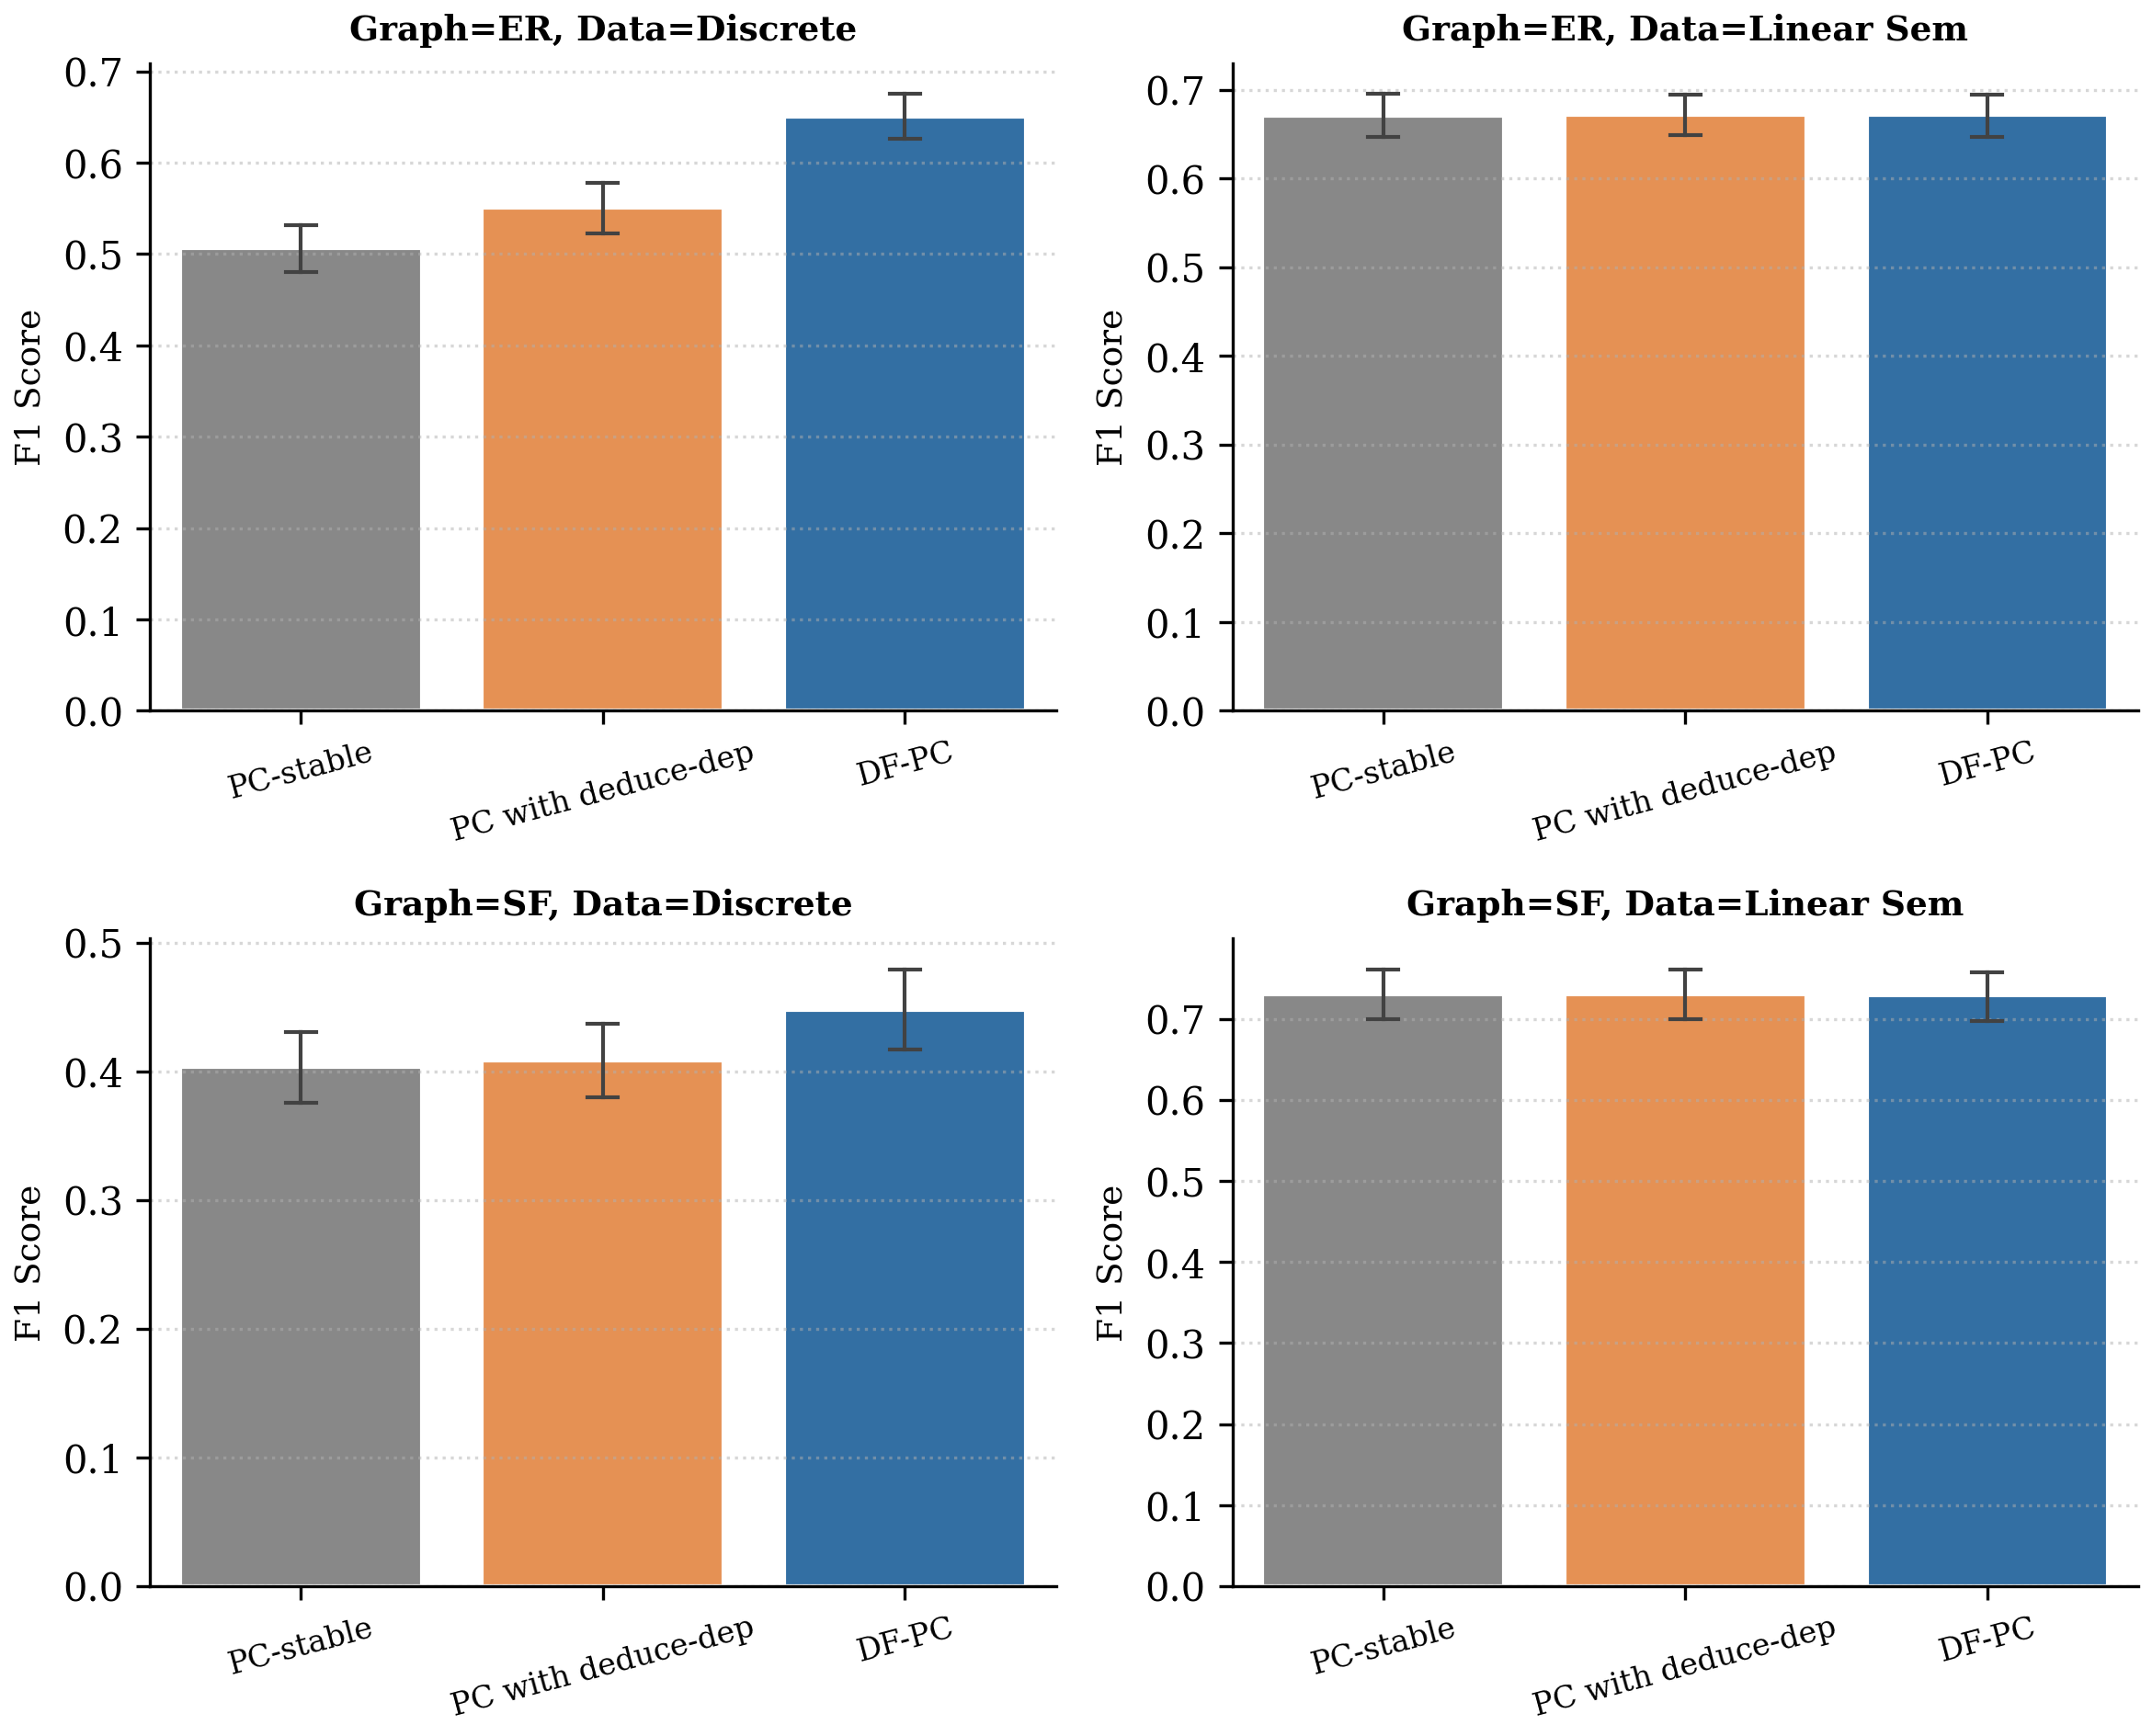
\includegraphics[width=\textwidth]{plots/exp1_f1.png}
    \caption{\textbf{Exp 1: F1 Score Comparison.} F1 score for various algorithms across ER and SF graph topologies with discrete and linear Gaussian data. The experiments are conducted with 20 nodes, 5000 samples, and an average degree of 4. Bars represent the mean across 30 independent trials with unique random seeds, and error bars indicate the 95\% confidence interval (CI).}
    \label{fig:exp1_f1}
\end{figure}

\begin{figure}[htbp]
    \centering
    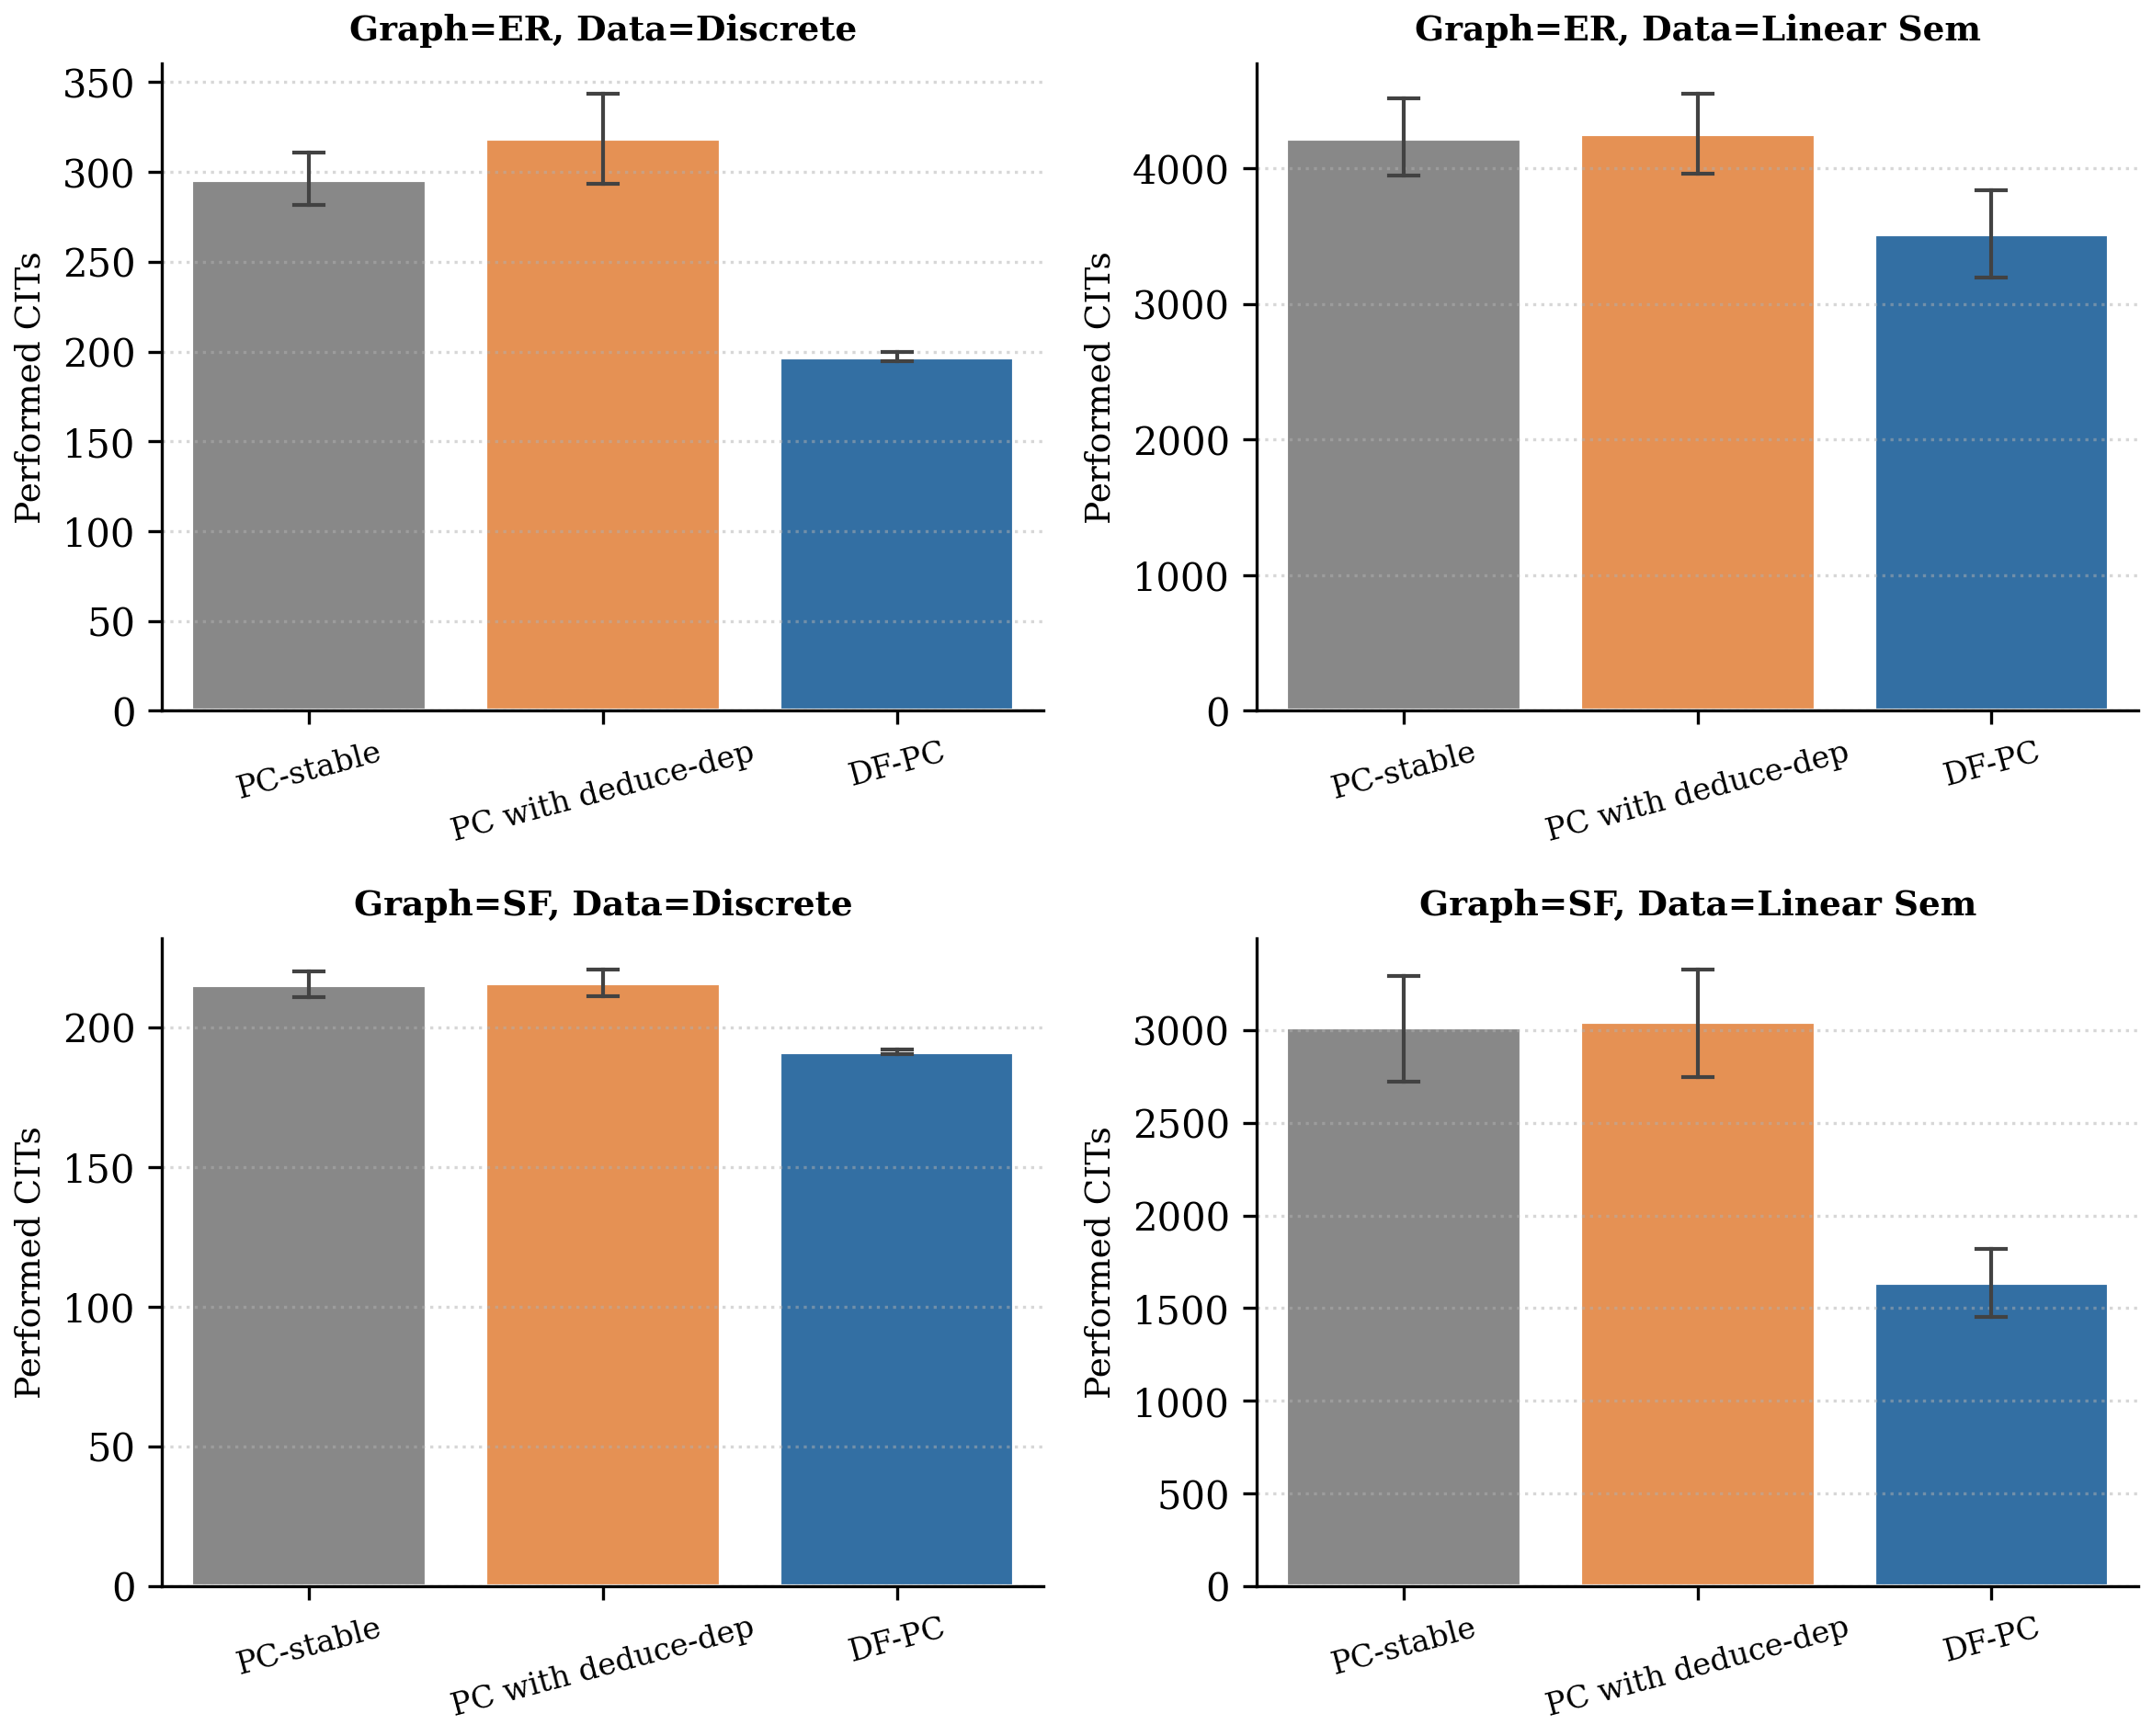
\includegraphics[width=\textwidth]{plots/exp1_performed_cits.png}
    \caption{\textbf{Exp 1: Count of Performed CITs.} The number of Conditional Independence Tests (CITs) executed by each algorithm. The setup uses 20 nodes, 5000 samples, and an average degree of 4. Error bars indicate the 95\% CI calculated over 30 trials.}
    \label{fig:exp1_cits}
\end{figure}

\begin{figure}[htbp]
    \centering
    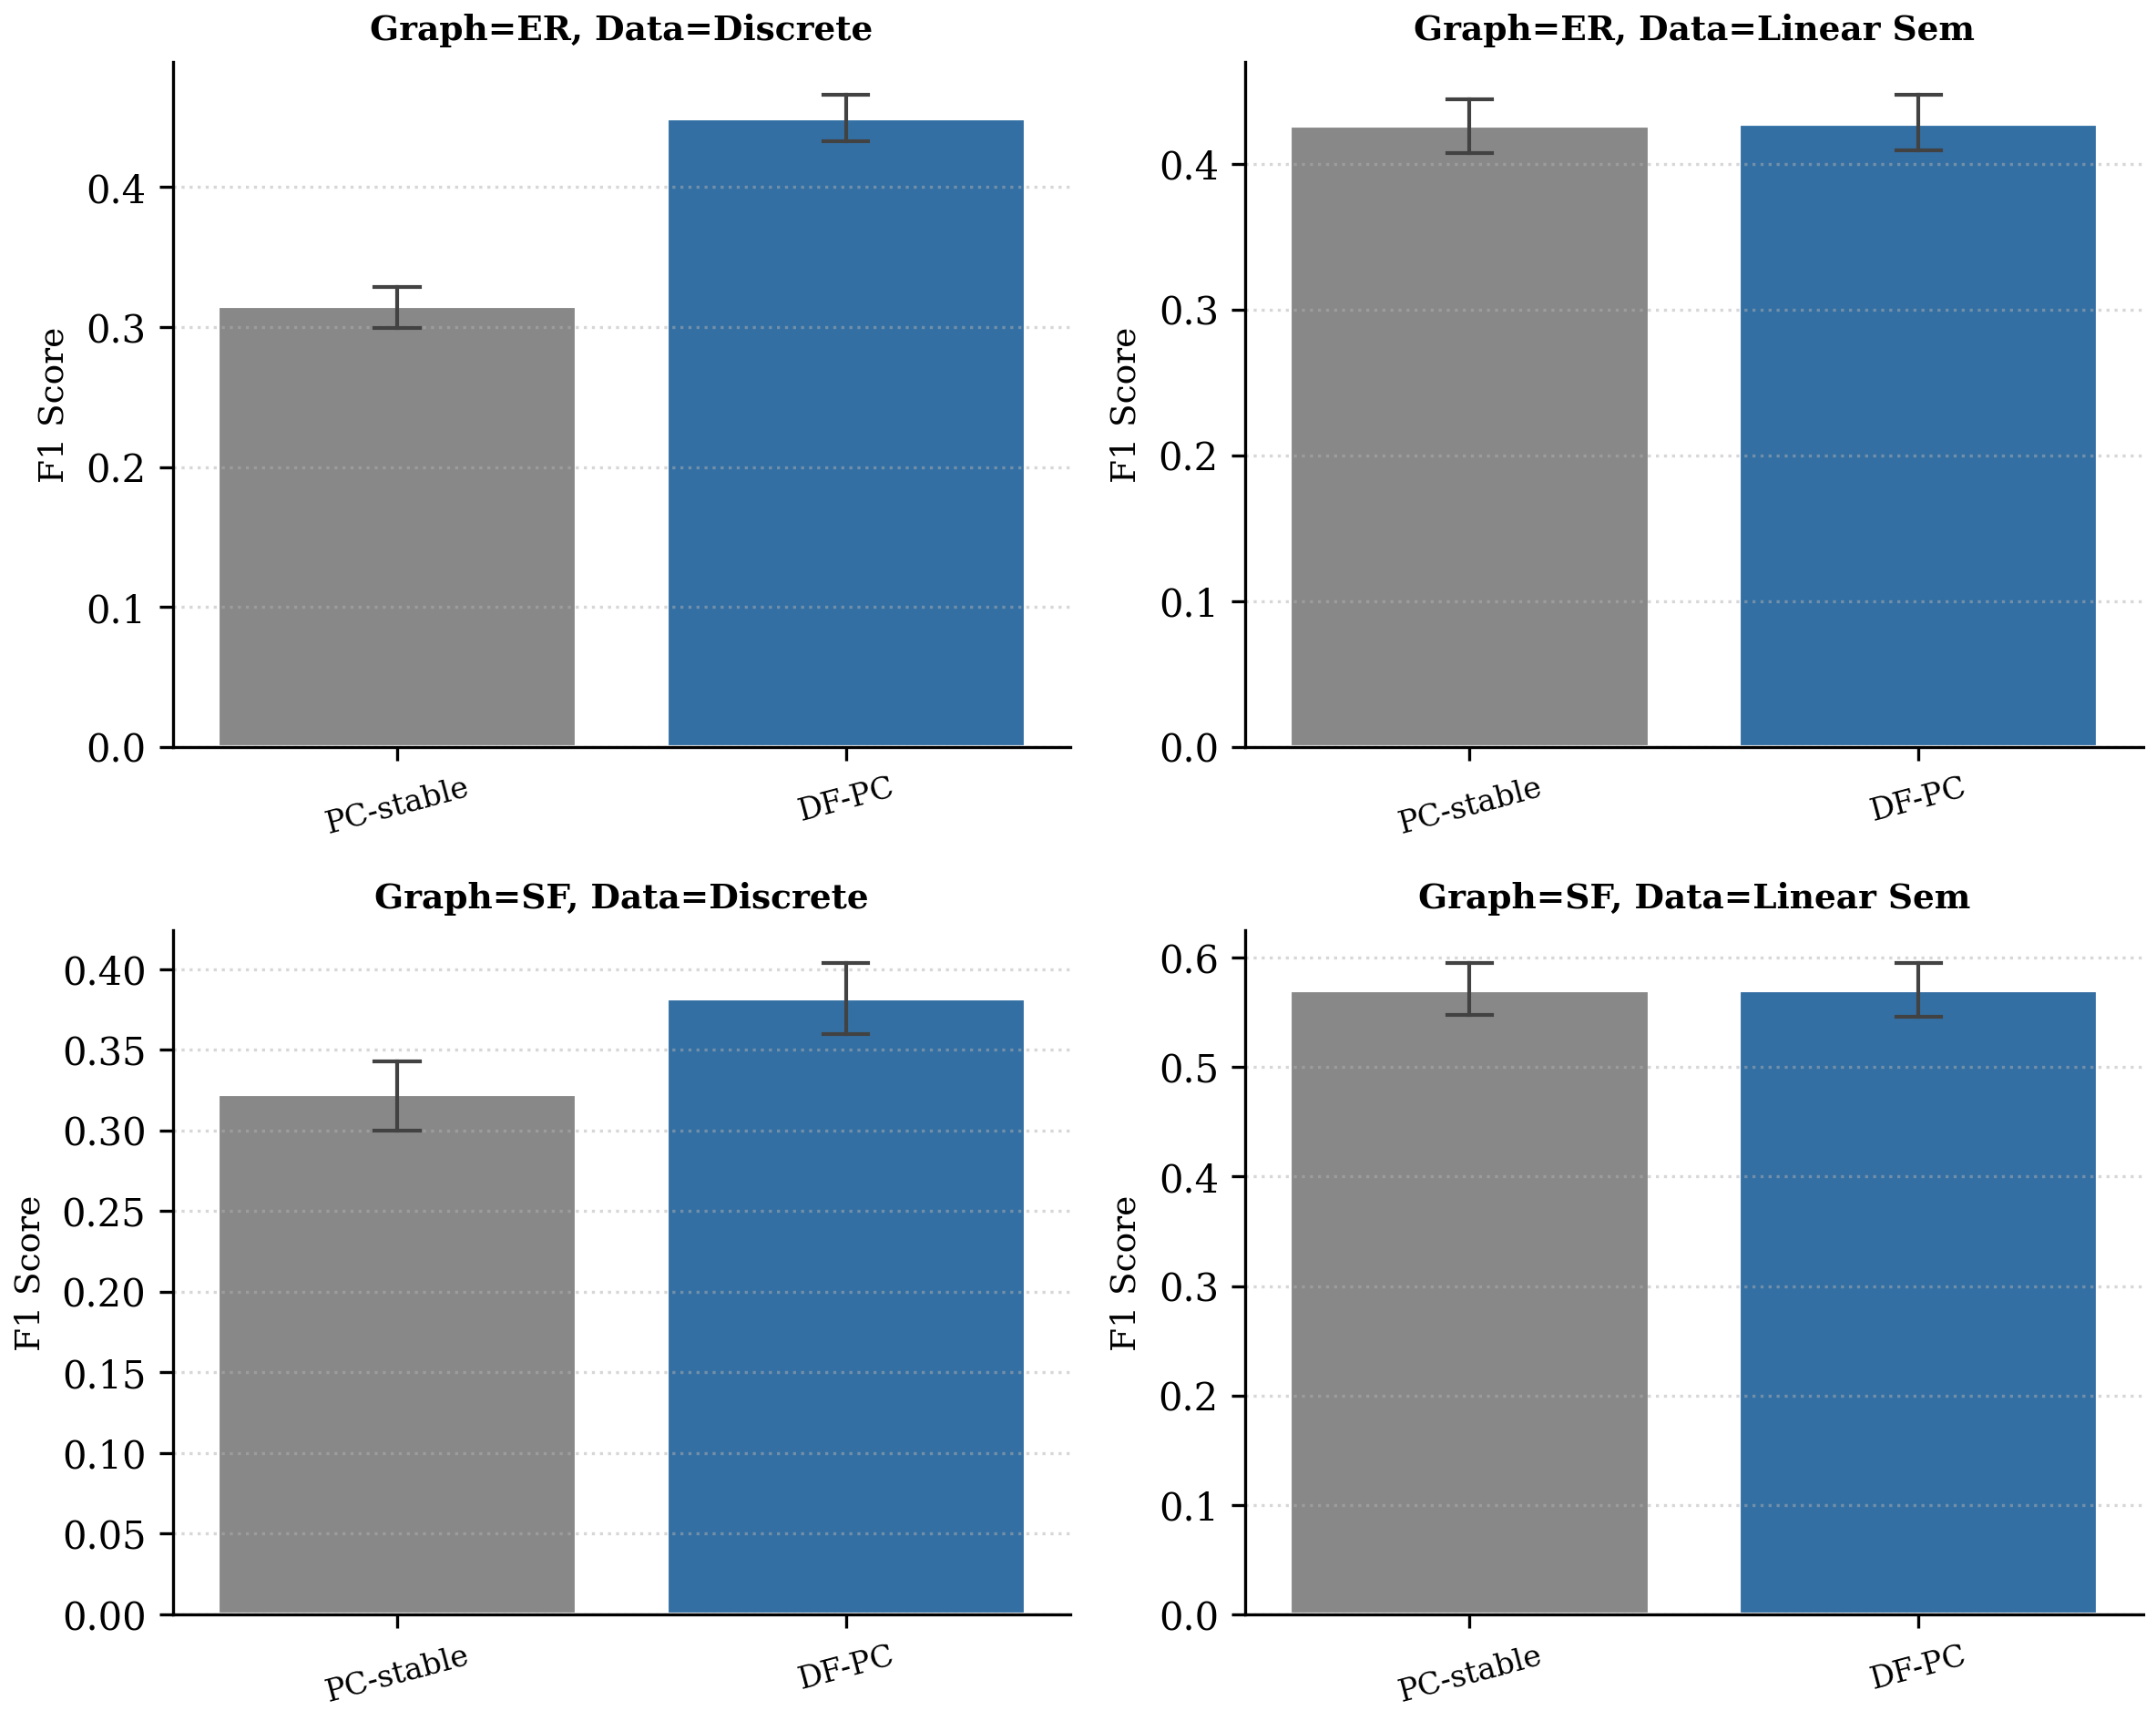
\includegraphics[width=\textwidth]{plots/exp2_f1.png}
    \caption{\textbf{Exp 2: Performance in High-Density Settings (F1).} F1 score on graphs with 30 nodes, 5000 samples, and an average degree of 6. Error bars represent 95\% CI across 30 independent trials.}
    \label{fig:exp2_f1}
\end{figure}

\begin{figure}[htbp]
    \centering
    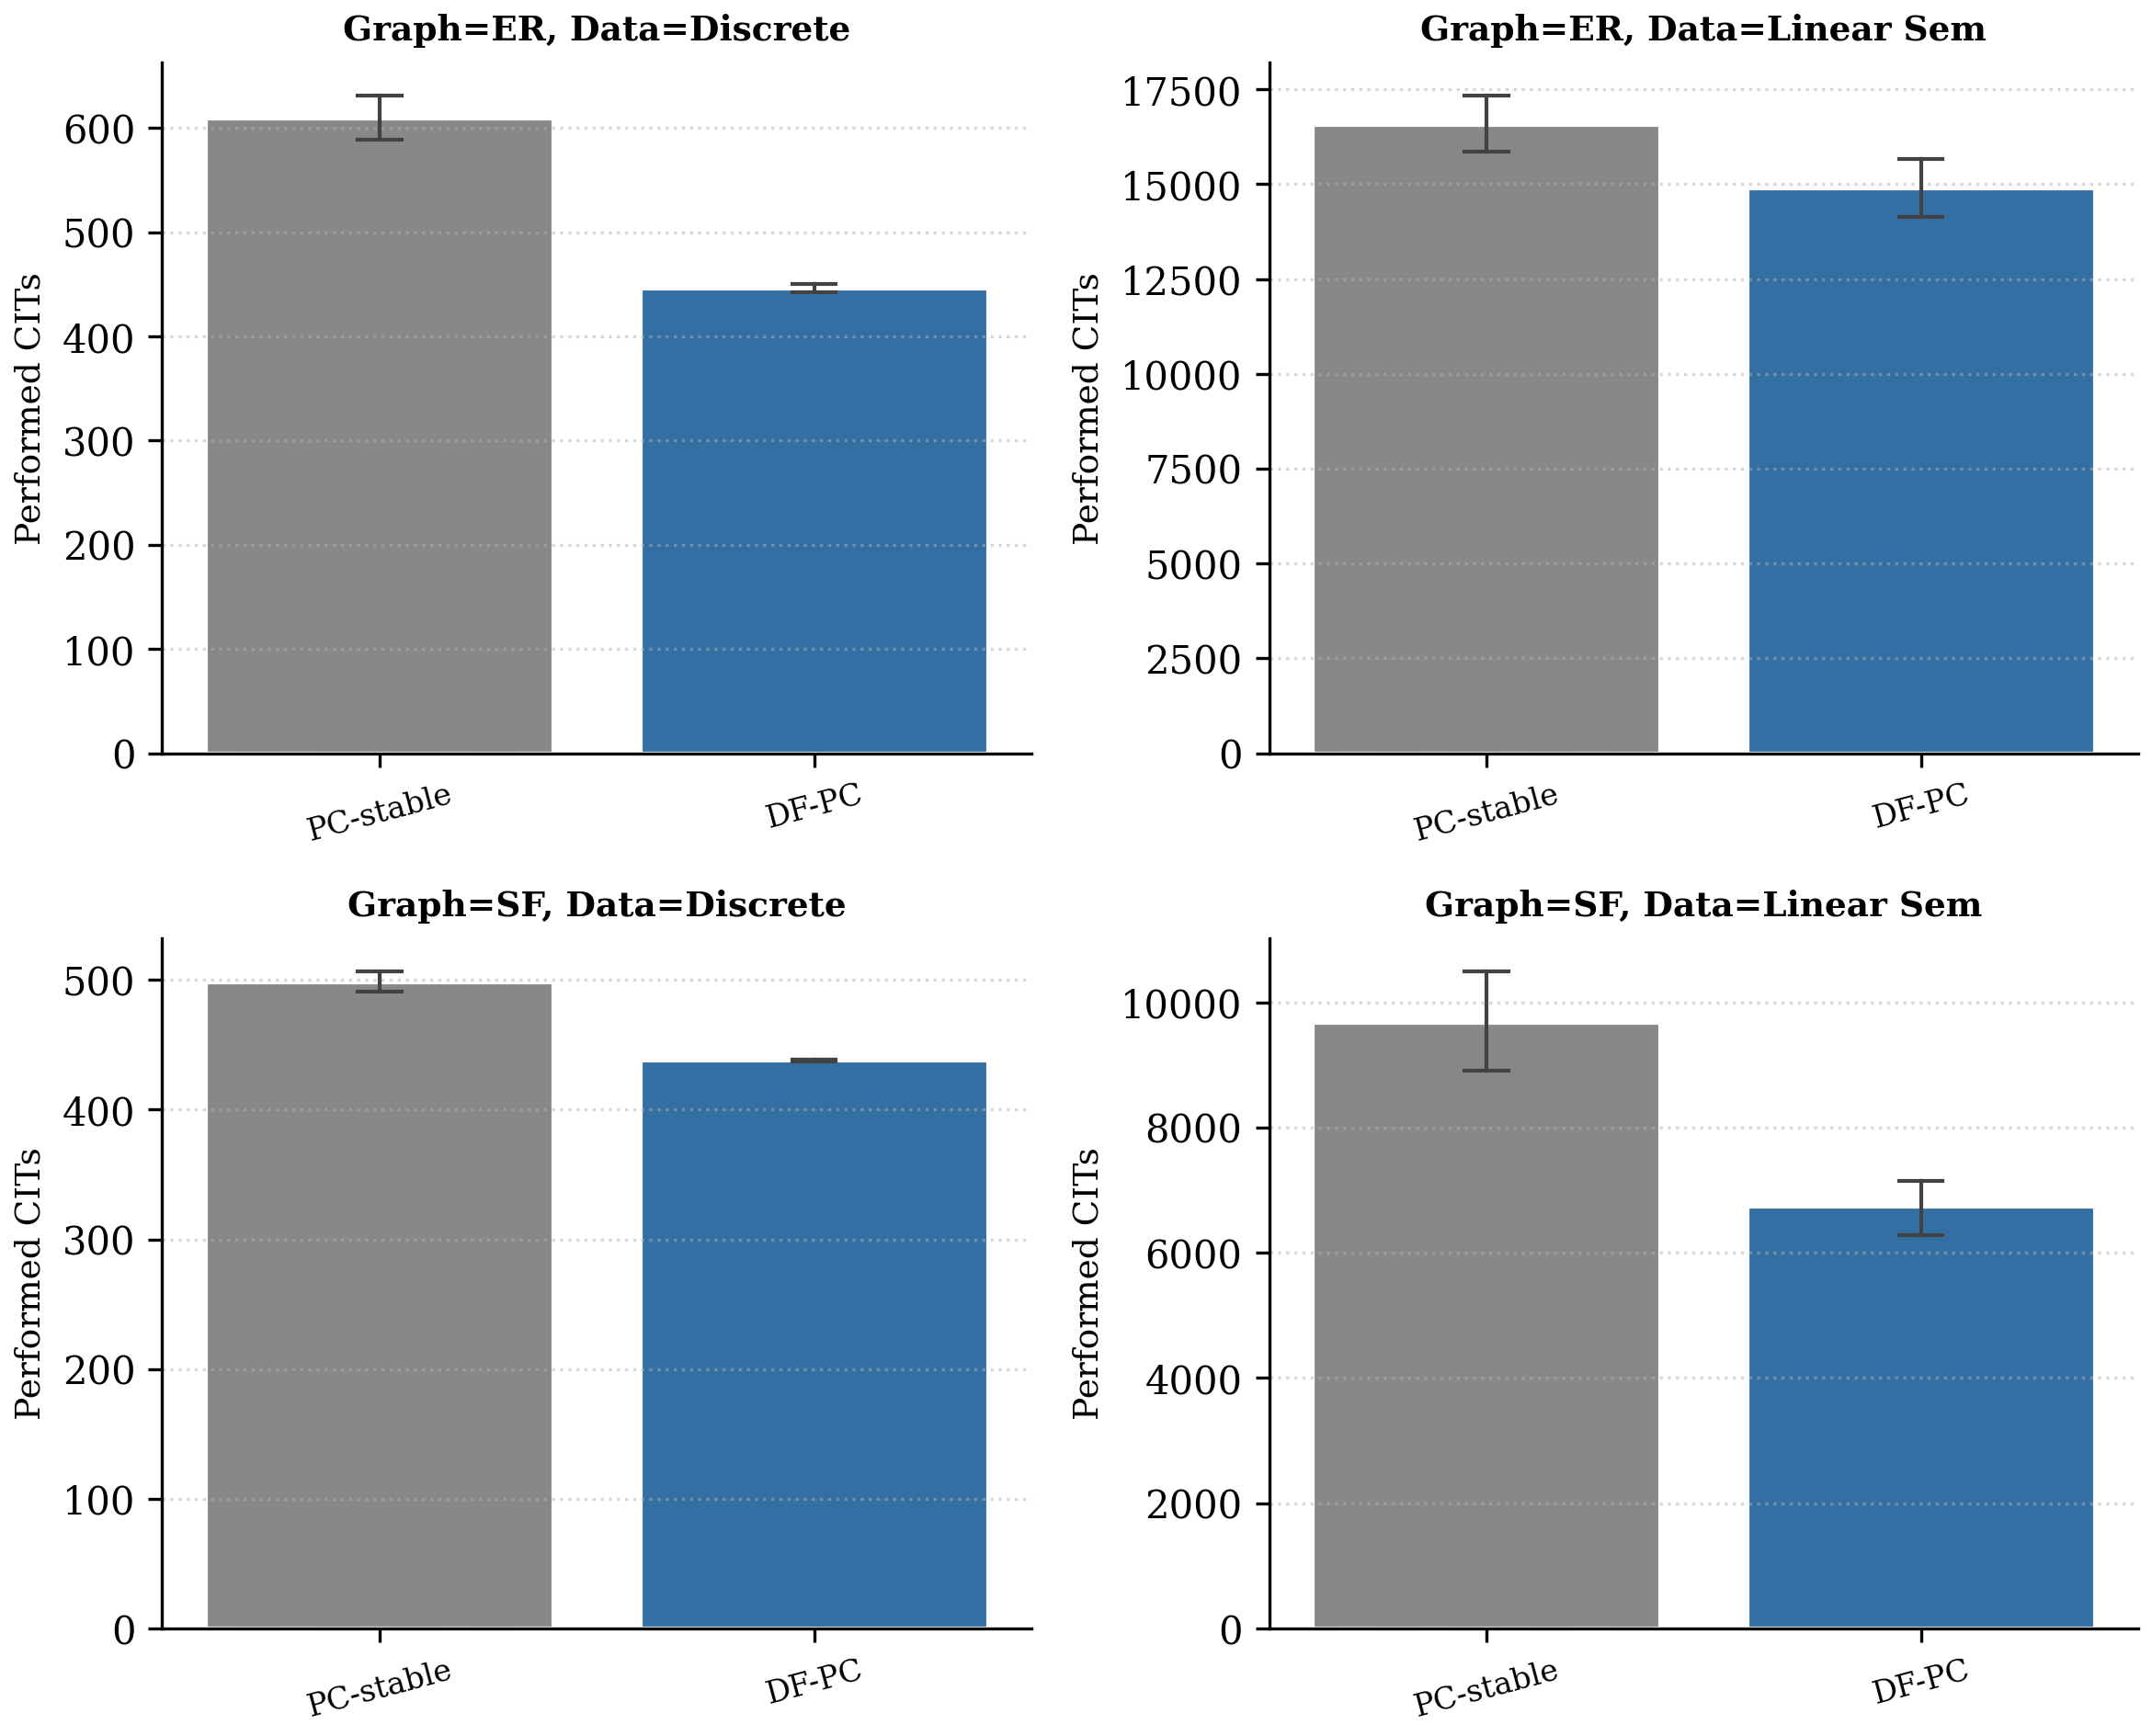
\includegraphics[width=\textwidth]{plots/exp2_performed_cits.png}
    \caption{\textbf{Exp 2: CIT Counts in High-Density Settings.} Total performed CITs for 30 nodes and 5000 samples with an average degree of 6. Error bars denote 95\% CI based on 30 trials.}
    \label{fig:exp2_cits}
\end{figure}

\newpage
\begin{figure}[htbp]
    \centering
    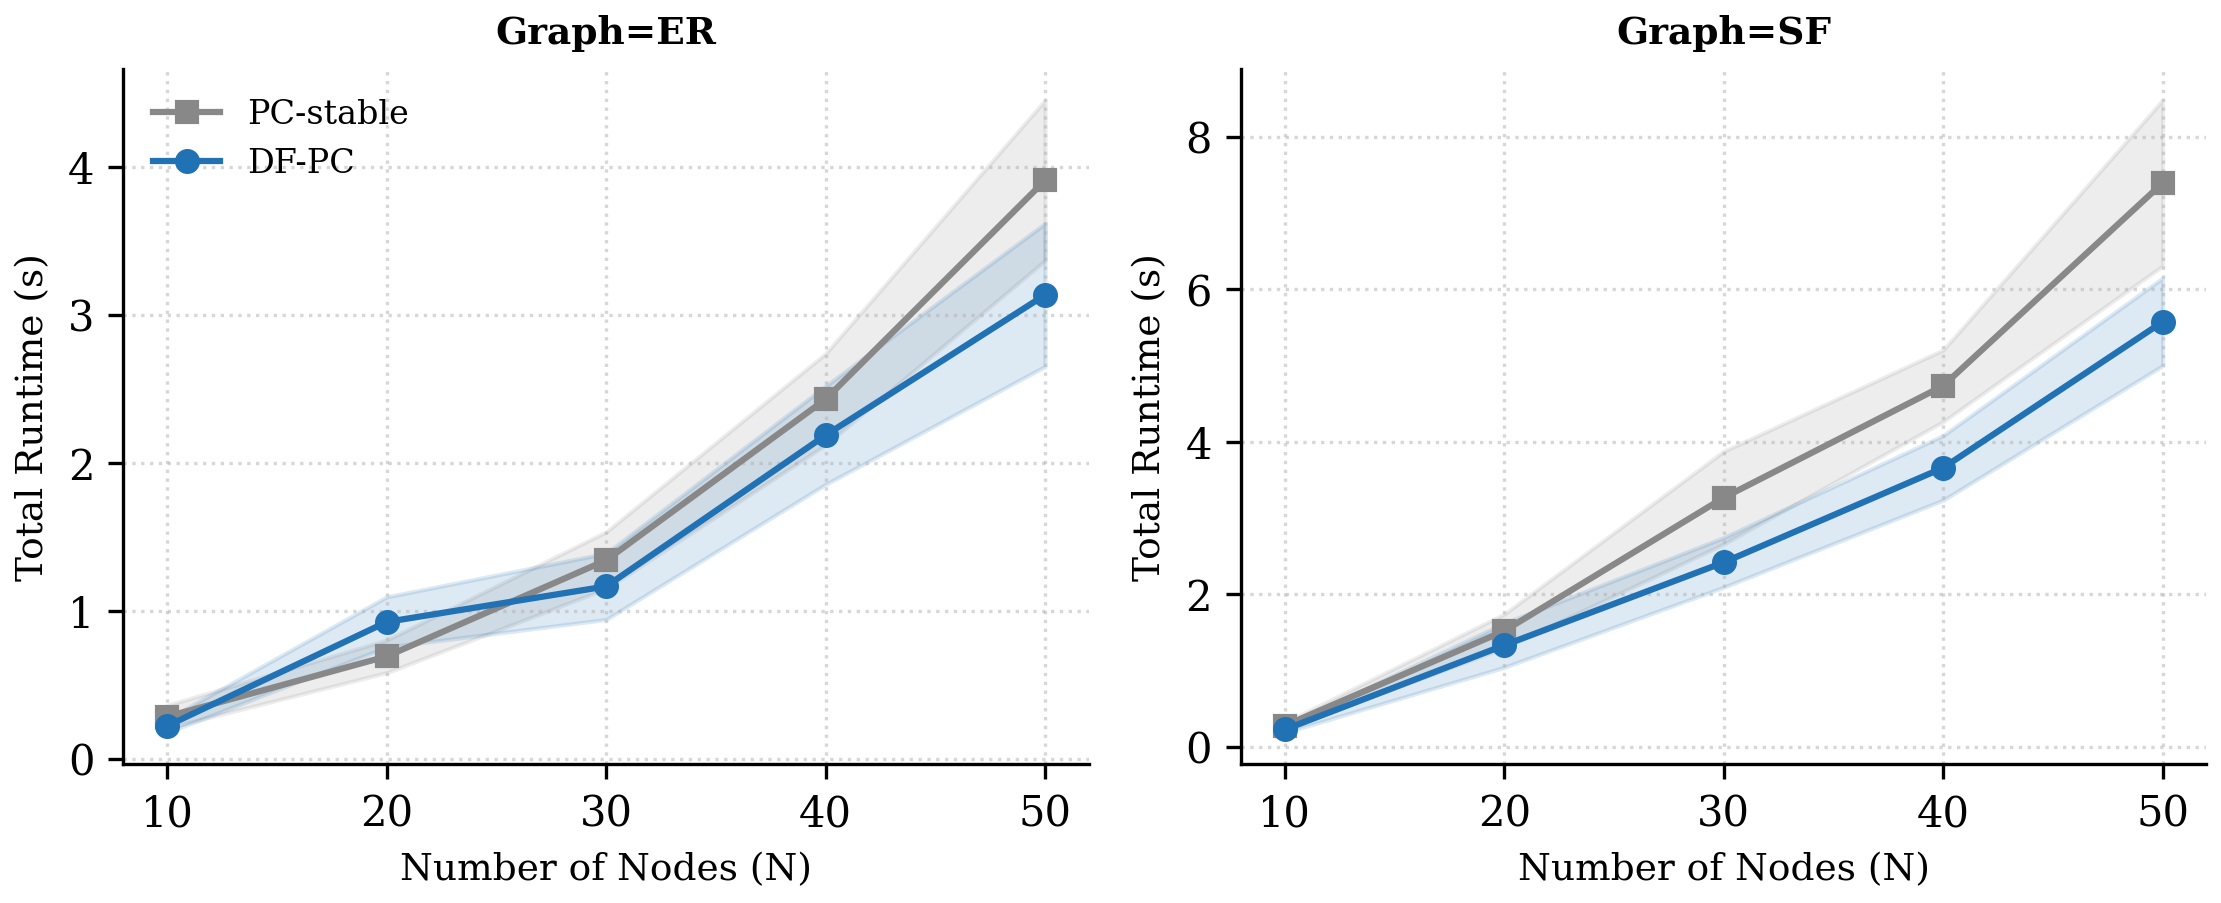
\includegraphics[width=\textwidth]{plots/exp3_runtime_nodes.png}
    \caption{\textbf{Exp 3: Runtime Scaling across Node Counts.} Total execution time in seconds as the number of nodes $N$ scales from 20 to 50, with an average degree of 3 and 5000 samples across Linear SEM data. Markers indicate the mean, and error bars represent the 95\% CI over 30 trials.}
    \label{fig:exp3_runtime_nodes}
\end{figure}

\begin{figure}[htbp]
    \centering
    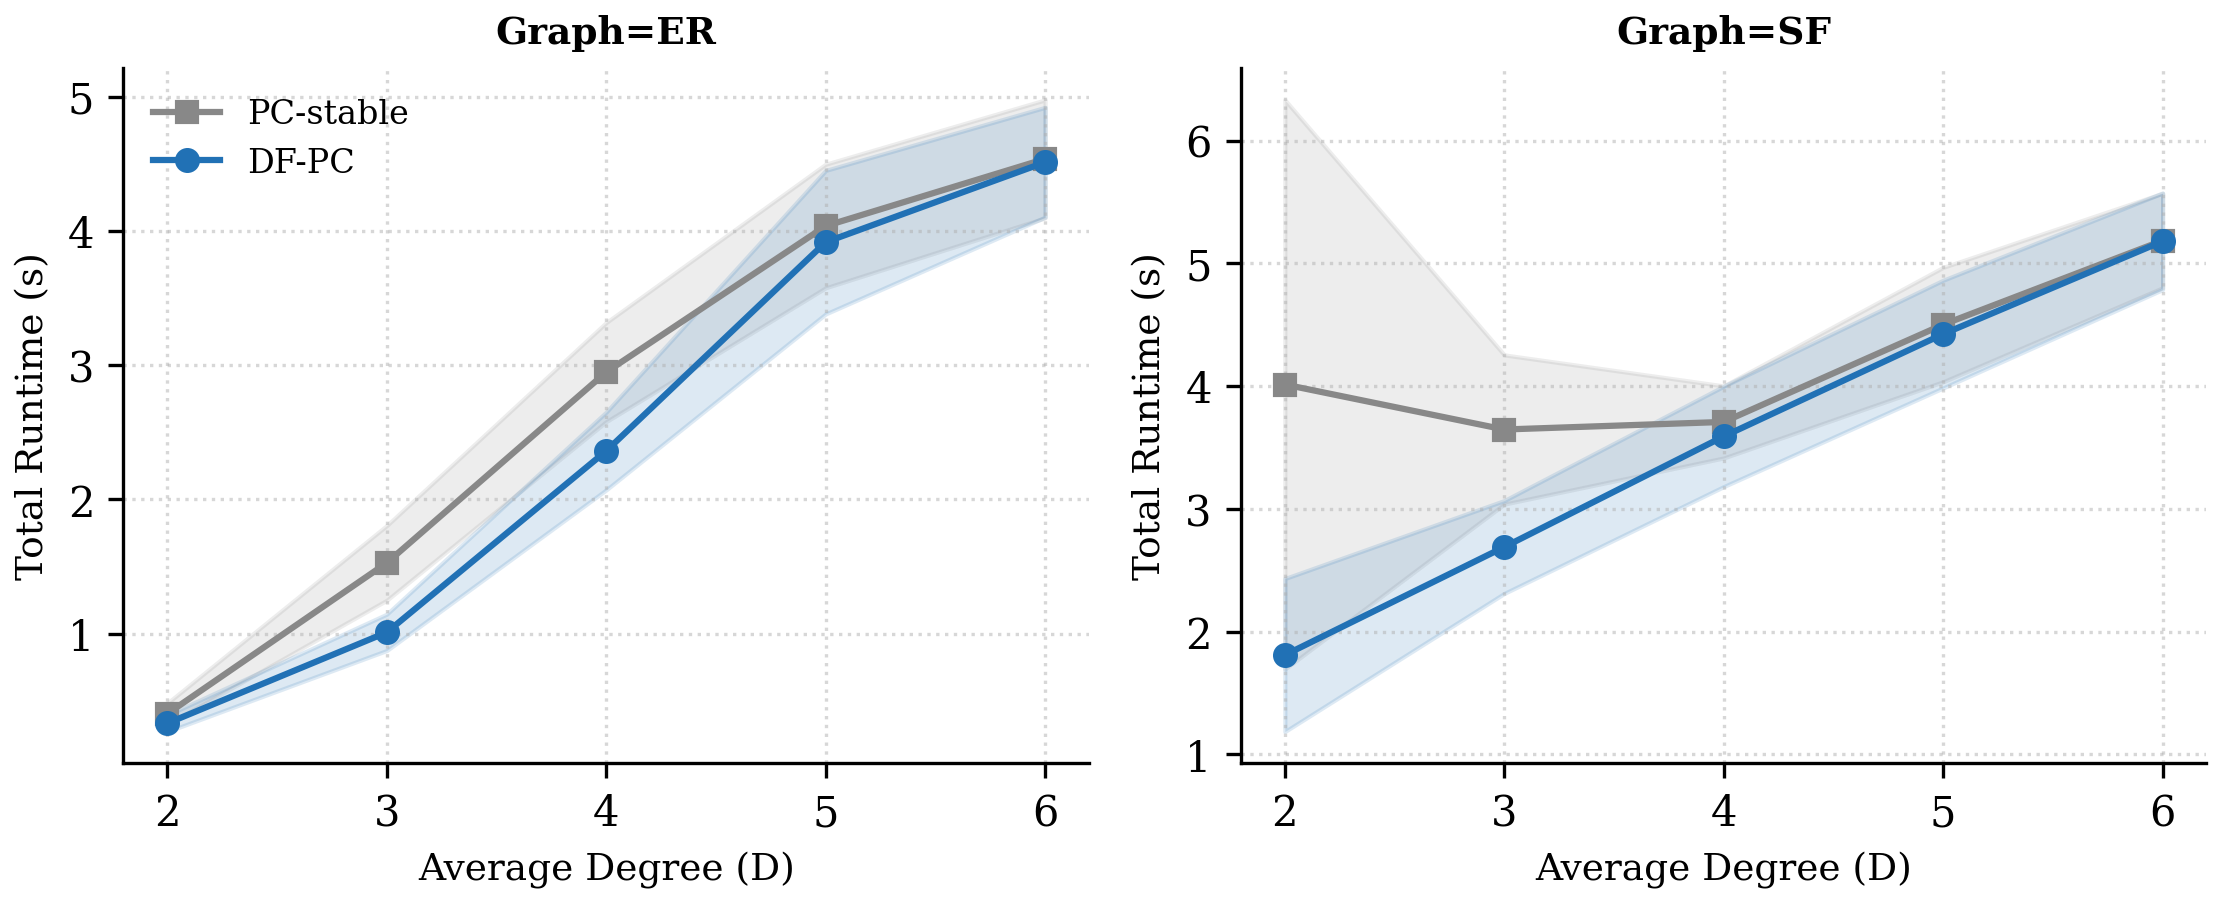
\includegraphics[width=\textwidth]{plots/exp3_runtime_density.png}
    \caption{\textbf{Exp 3: Runtime Scaling across Graph Density.} Execution time as the average degree $d$ scales from 2 to 6 for a 30-node graph with 5000 samples in Linear SEM data. Error bars indicate 95\% CI across 30 independent trials.}
    \label{fig:exp3_runtime_density}
\end{figure}

\begin{figure}[htbp]
    \centering
    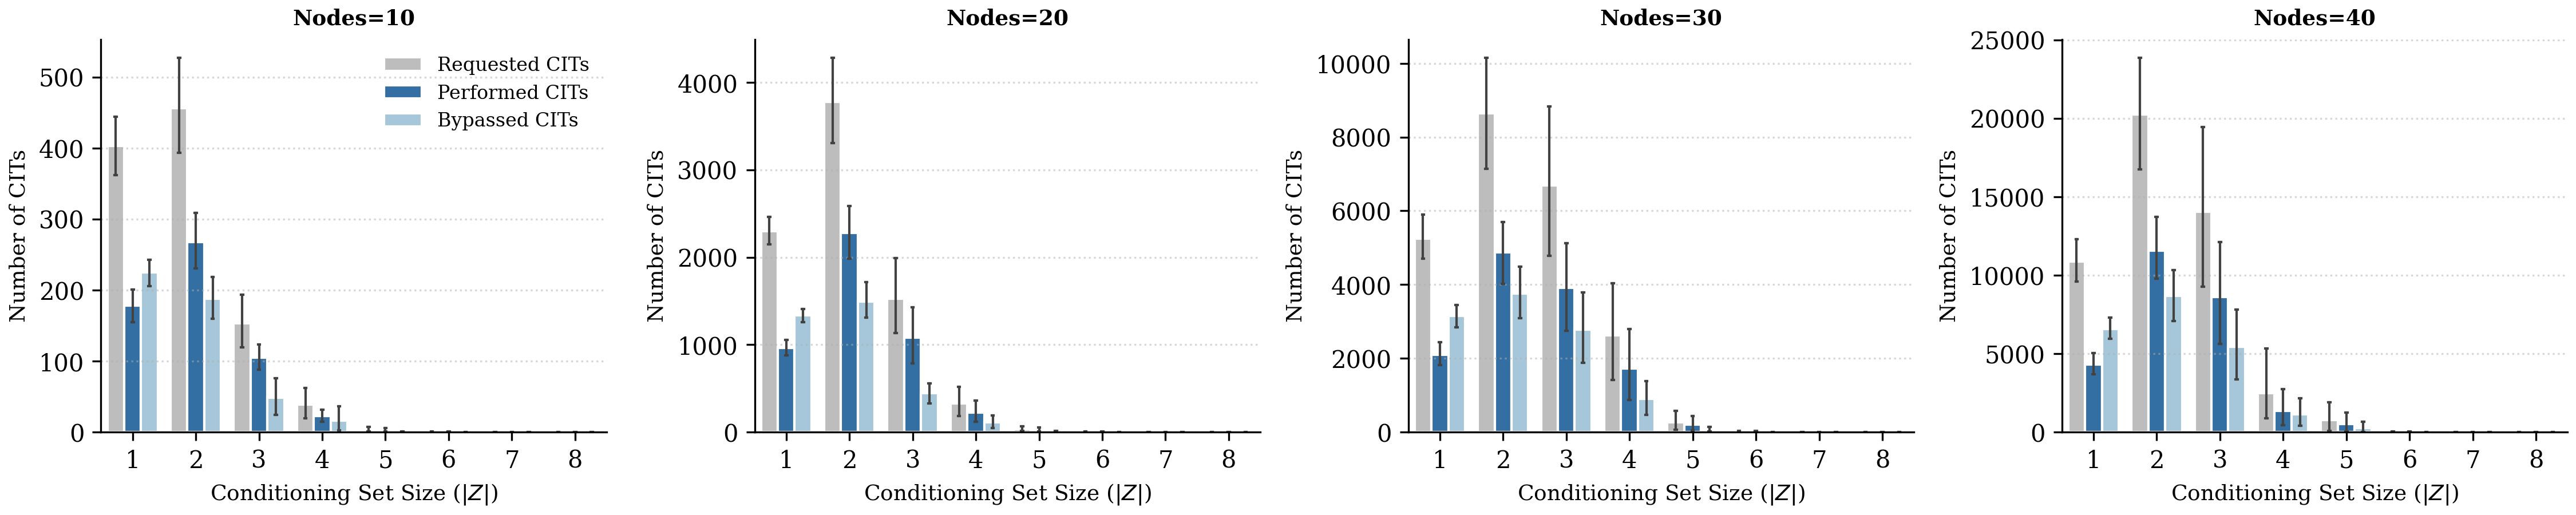
\includegraphics[width=\textwidth]{plots/exp4_save_CIT_nodes.png}
    \caption{\textbf{Exp 4: CIT Skip Analysis across Node Counts.} Decomposition of CIT requests categorized by conditioning set size $|Z|$ for ER graphs with an average degree of 3 using an oracle CIT. \textit{Requested CITs} denotes total tests requested by the algorithm, \textit{Performed CITs} denotes tests actually run by DF-PC, and \textit{Bypassed CITs} denotes tests skipped via logical deduction. Error bars indicate 95\% CI based on 30 seeds.}
    \label{fig:exp4_save_nodes}
\end{figure}

\begin{figure}[htbp]
    \centering
    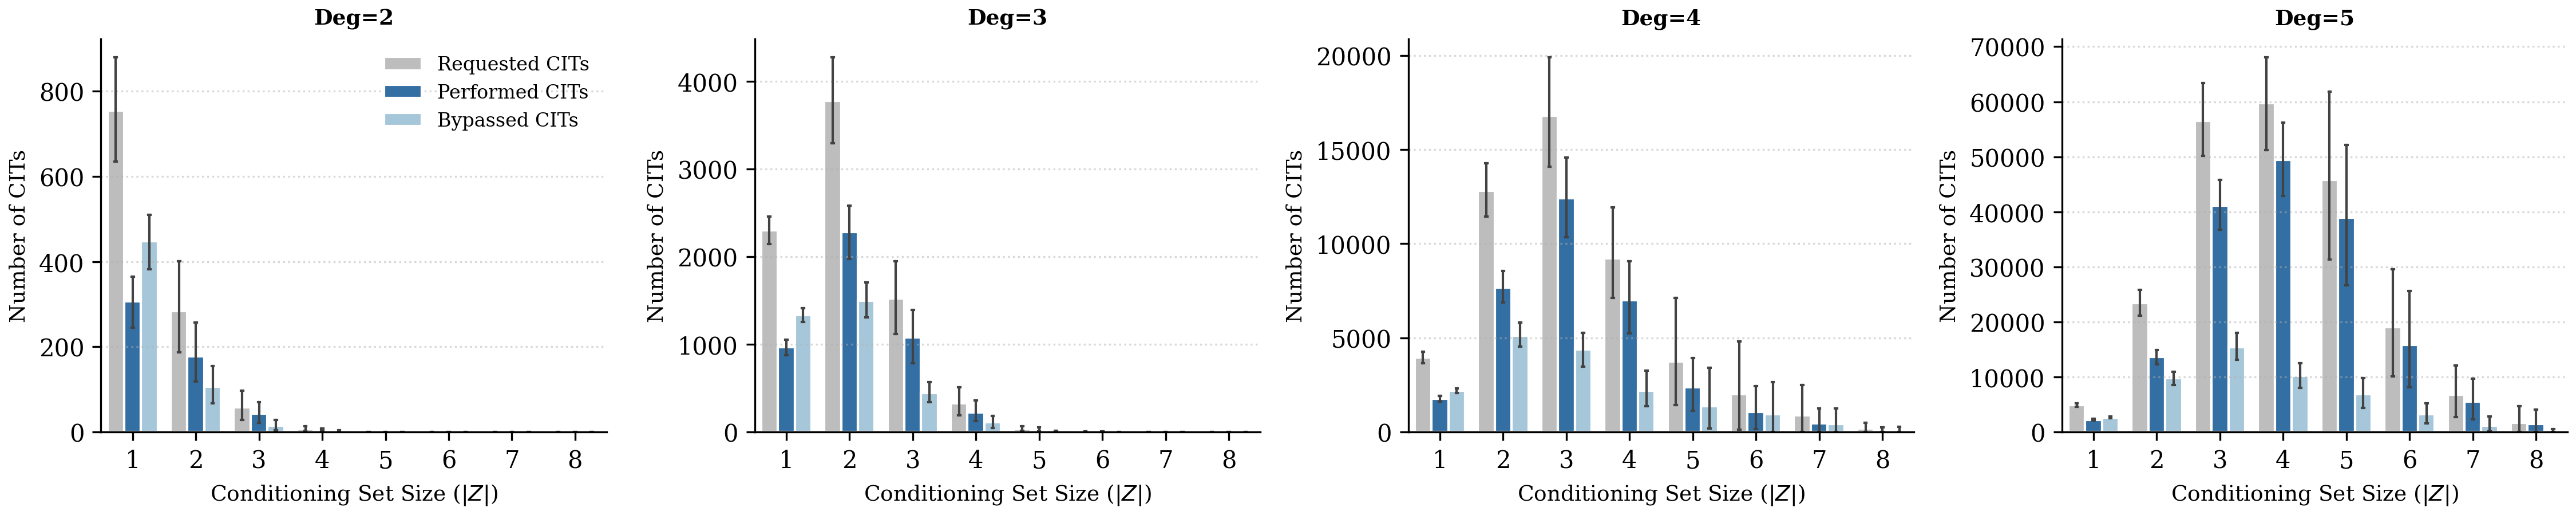
\includegraphics[width=\textwidth]{plots/exp4_save_CIT_density.png}
    \caption{\textbf{Exp 4: CIT Skip Analysis across Graph Density.} Categorized CIT counts as graph density increases from average degree 2 to 5 for an ER graph with 20 nodes using an oracle CIT. Error bars indicate 95\% CI across 30 trials.}
    \label{fig:exp4_save_density}
\end{figure}

\begin{figure}[htbp]
    \centering
    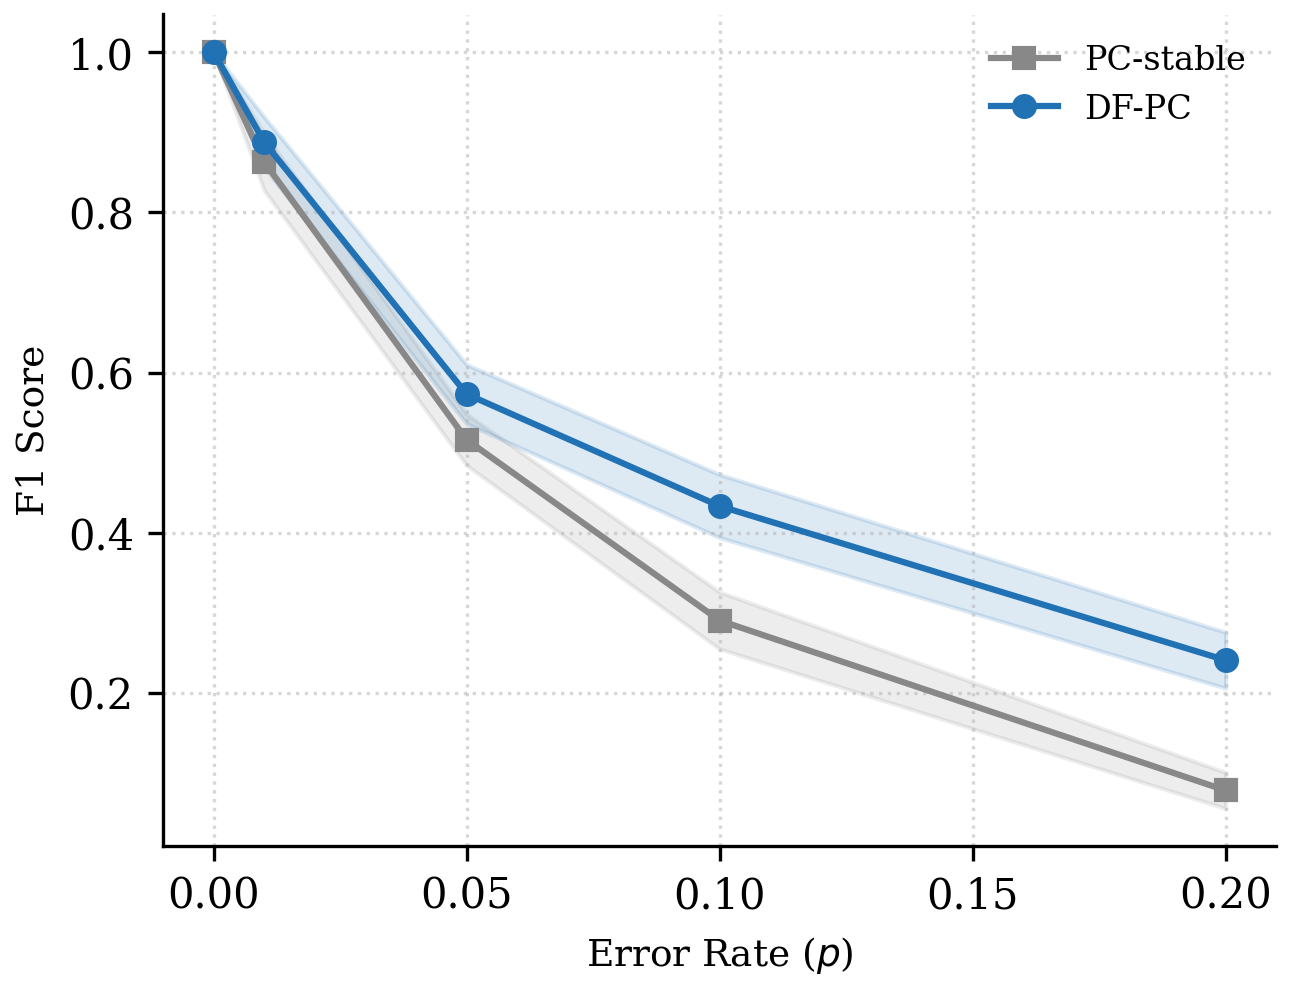
\includegraphics[width=0.7\textwidth]{plots/exp5_robustness.png}
    \caption{\textbf{Exp 5: Robustness against Low-Order CIT Errors.} F1 score when random errors with rate $p$ are injected into low-order oracle CITs ($|Z| \le 1$) for a graph with 20 nodes and an average degree of 3 in an ER topology. Error bars indicate 95\% CI derived from 30 independent trials.}
    \label{fig:exp5_robustness}
\end{figure}
